\chapter{6.13 习题}
%---------- 1 ----------------
\begin{flushleft}
1. 写出下面顶点结构的 D3D12\_INPUT\_ELEMENT\_DESC 数组:
\end{flushleft}
\begin{lstlisting}
struct Vertex
{
    XMFLOAT3 Pos;
    XMFLOAT3 Tangent;
    XMFLOAT3 Normal;
    XMFLOAT2 Tex0;
    XMFLOAT2 Tex1;
    XMCOLOR  Color;
};
\end{lstlisting}
\begin{flushleft}
解:\\
\end{flushleft}
\begin{lstlisting}
std::vector<D3D12_INPUT_ELEMENT_DESC> mInputLayout;
mInputLayout = {
    { "POSITION", 0, DXGI_FORMAT_R32G32B32_FLOAT, 0, 0, 
                  D3D12_INPUT_CLASSIFICATION_PER_VERTEX_DATA, 0 },
    { "TANGENT",  0, DXGI_FORMAT_R32G32B32_FLOAT, 0, 12, 
                  D3D12_INPUT_CLASSIFICATION_PER_VERTEX_DATA, 0 },
    { "NORMAL",   0, DXGI_FORMAT_R32G32B32_FLOAT, 0, 24, 
                  D3D12_INPUT_CLASSIFICATION_PER_VERTEX_DATA, 0 },
    { "TEXCOORD", 0, DXGI_FORMAT_R32G32_FLOAT, 0, 36, 
                  D3D12_INPUT_CLASSIFICATION_PER_VERTEX_DATA, 0 },
    { "TEXCOORD", 1, DXGI_FORMAT_R32G32_FLOAT, 0, 44, 
                  D3D12_INPUT_CLASSIFICATION_PER_VERTEX_DATA, 0 },
    { "COLOR",    0, DXGI_FORMAT_R8G8B8A8_UINT, 0, 52, 
                  D3D12_INPUT_CLASSIFICATION_PER_VERTEX_DATA, 0 }
};
\end{lstlisting}

%---------- 2 ----------------
\begin{flushleft}
~\\
2. 重写Box DEMO,这次使用 2 个顶点缓冲区(2个输入槽)给管道提供顶点数据。一个缓冲区存储位置元素,另一个存储存储颜色元素。下面给定两个分开的顶点数据结构:\\
\end{flushleft}
\begin{lstlisting}
struct VPosData
{
    XMFLOAT3 Pos;
};

struct VColorData
{
    XMFLOAT4 Color;
};
\end{lstlisting}
\begin{flushleft}
位置元素挂在输入槽0上,颜色元素挂在输入槽1上。此外还需注意 D3D12\_INPUT\_ELEMENT\_DESC::AlignedByteOffset 对于两个元素来说都是0;然后使用 ID3D12CommandList::IASetVertexBuffers 方法来将缓冲区绑定到槽0和槽1。然后,Direct3D将使用来自不同输入槽的元素来组合顶点。 这可以用作优化。 例如,在阴影映射算法中,我们需要每帧绘制两次场景:一次从光源的角度(阴影传递),一次从主摄像头的角度(主传递)。 阴影传递仅需要位置数据和纹理坐标(对于经过alpha测试的几何体)。 因此我们可以将顶点数据分成两个槽:一个槽包含位置和纹理坐标,另一个槽包含其他顶点属性(例如,法线和切线矢量)。 现在我们可以轻松地仅在阴影传递所需的顶点数据中流动(位置和纹理坐标),从而为阴影传递节省数据带宽。 主渲染过程将使用两个顶点输入槽来获取所需的所有顶点数据。 为了提高性能,建议最小化用于小于或等于3的小数字的输入槽数。\\
\end{flushleft}
\begin{flushleft}
解:\\
要点:\\
\begin{itemize}
  \item 1. 调用 IASetVertexBuffers 指定输入槽用于提供数据
  \item 2. D3D12\_INPUT\_LAYOUT\_DESC的D3D12\_INPUT\_ELEMENT\_DESC 结构中的 inputSlot 用于指定 hlsl 中对应的 SemanticName 输入参数来自于哪个槽。
  \item 3. 1,2 提供了 Color 和 Pos 绑定在一起的依据。在顶点着色器阶段,能顺利将 Color 和 Pos 整合成 VertexIn。
\end{itemize}
需要修改的部分源码如下:\\
\end{flushleft}
\begin{lstlisting}
// chapter 6: BoxApp.cpp 修改
// 下面修改满足题目要求外,新增了一个三角形平面
// ...code...
struct VPosData
{
    XMFLOAT3 Pos;
};

struct VColorData
{
    XMFLOAT4 Color;
};

// ...code...

class BoxApp : public D3DApp
{
    // ...code...

    // 这里的 mTheta 和 mPhi 是初始时,摄像机对准的角度
    float mTheta = 1.5f*XM_PI; // 左右角度
    float mPhi = XM_PIDIV4;    // 上下角度
    // 摄像机到目标原点的距离,也相当于屏幕横坐标的大小;
    // 控制半径,能让立方体放大缩小,半径越大,立方体越小
    float mRadius = 10.0f;

    // ...code...
};

// ...code...

void BoxApp::Draw(const GameTimer& gt)
{
    // ...code...
    
    // 重要修改在这里

    // Position slot 0
    mCommandList->IASetVertexBuffers(0, 1, &mGeoPos->VertexBufferView());
    // Color: slot 1
    mCommandList->IASetVertexBuffers(1, 1, &mGeoColor->VertexBufferView());
    mCommandList->IASetIndexBuffer(&mGeoPos->IndexBufferView());
    mCommandList->IASetPrimitiveTopology(
                      D3D11_PRIMITIVE_TOPOLOGY_TRIANGLELIST);

    mCommandList->SetGraphicsRootDescriptorTable(0, 
                      mCbvHeap->GetGPUDescriptorHandleForHeapStart());

    SubmeshGeometry boxmesh = mGeoPos->DrawArgs["box"];
    mCommandList->DrawIndexedInstanced(boxmesh.IndexCount, 1,
                      boxmesh.StartIndexLocation, 
                      boxmesh.BaseVertexLocation, 0);

    SubmeshGeometry trianglemesh = mGeoPos->DrawArgs["triangle"];
    mCommandList->DrawIndexedInstanced(trianglemesh.IndexCount, 1, 
                      trianglemesh.StartIndexLocation, 
                      trianglemesh.BaseVertexLocation, 0);

    // ...code...
}

// ...code...

void BoxApp::BuildShadersAndInputLayout()
{
    HRESULT hr = S_OK;

    mvsByteCode = d3dUtil::CompileShader(L"Shaders\\color.hlsl", 
                      nullptr, "VS", "vs_5_0");
    mpsByteCode = d3dUtil::CompileShader(L"Shaders\\color.hlsl", 
                      nullptr, "PS", "ps_5_0");

    // 重要修改在这里: COLOR 的 InputSlot 为 1,AlignedByteOffset 为 0
    mInputLayout = {
        { "POSITION", 0, DXGI_FORMAT_R32G32B32_FLOAT, 0, 0, 
                      D3D12_INPUT_CLASSIFICATION_PER_VERTEX_DATA, 0 },
        { "COLOR",    0, DXGI_FORMAT_R32G32B32A32_FLOAT, 1, 0, 
                      D3D12_INPUT_CLASSIFICATION_PER_VERTEX_DATA, 0 }
    };
}

// 重要修改在这里:新增了三角形,position 数据和 color 数据分开
void BoxApp::BuildBoxGeometry()
{
    std::array<VPosData, 11> posVertices = {
        // 正立方体 position
        XMFLOAT3(-1.0f, -1.0f, -1.0f),  // 0
        XMFLOAT3(-1.0f, +1.0f, -1.0f),  // 1
        XMFLOAT3(+1.0f, +1.0f, -1.0f),  // 2
        XMFLOAT3(+1.0f, -1.0f, -1.0f),  // 3
        XMFLOAT3(-1.0f, -1.0f, +1.0f),  // 4
        XMFLOAT3(-1.0f, +1.0f, +1.0f),  // 5
        XMFLOAT3(+1.0f, +1.0f, +1.0f),  // 6
        XMFLOAT3(+1.0f, -1.0f, +1.0f),  // 7
        // 三角形 color
        XMFLOAT3(2.0f, 1.0f, -2.0f),    // 0
        XMFLOAT3(2.0f, +3.0f,-2.0f),    // 1
        XMFLOAT3(+3.0f, +3.0f, -2.0f)   // 2
    };

    std::array<VColorData, 11> colorVertices = {
        // 正立方体 color
        XMFLOAT4(Colors::White),  // 0
        XMFLOAT4(Colors::Black),  // 1
        XMFLOAT4(Colors::Red),    // 2
        XMFLOAT4(Colors::Green),  // 3
        XMFLOAT4(Colors::Blue),   // 4
        XMFLOAT4(Colors::Yellow), // 5
        XMFLOAT4(Colors::Cyan),   // 6
        XMFLOAT4(Colors::Magenta),// 7
        // 三角形 color
        XMFLOAT4(Colors::Magenta), // 0
        XMFLOAT4(Colors::Blue),    // 1
        XMFLOAT4(Colors::Yellow)   // 2
    };

    std::array<std::uint16_t, 39> indices = {
        // 正立方体面
        // front face
        0, 1, 2,
        0, 2, 3,

        // back face
        4, 6, 5,
        4, 7, 6,

        // left face
        4, 5, 1,
        4, 1, 0,

        // right face
        3, 2, 6,
        3, 6, 7,

        // top face
        1, 5, 6,
        1, 6, 2,

        // bottom face
        4, 0, 3,
        4, 3, 7, // indexCount:36

        /*
        因为 DrawIndexedInstanced 里定义了 BaseVertexLocation,
        trianglemesh.BaseVertexLocation = 8,
        所以索引又从 0 开始来描绘三角形。即这里的 0,1,2 代表 vertices[8],[9],[10]
        */
        // 三角形
        0, 1, 2  // indexCount: 3
    };

    const UINT vbPosByteSize = 
              (UINT)posVertices.size() * sizeof(VPosData);
    const UINT vbColorByteSize = 
              (UINT)colorVertices.size() * sizeof(VColorData);
    const UINT ibByteSize = 
              (UINT)indices.size() * sizeof(std::uint16_t);

    mGeoPos = std::make_unique<MeshGeometry>();
    mGeoPos->Name = "GeoPos";

    mGeoColor = std::make_unique<MeshGeometry>();
    mGeoColor->Name = "GeoColor";

    ThrowIfFailed(D3DCreateBlob(vbPosByteSize, 
                  &mGeoPos->VertexBufferCPU));
    CopyMemory(mGeoPos->VertexBufferCPU->GetBufferPointer(), 
               posVertices.data(), vbPosByteSize);

    ThrowIfFailed(D3DCreateBlob(vbColorByteSize, 
                      &mGeoColor->VertexBufferCPU));
    CopyMemory(mGeoColor->VertexBufferCPU->GetBufferPointer(), 
               colorVertices.data(), vbColorByteSize);

    ThrowIfFailed(D3DCreateBlob(ibByteSize, 
                     &mGeoPos->IndexBufferCPU));
    CopyMemory(mGeoPos->IndexBufferCPU->GetBufferPointer(), 
                   indices.data(), ibByteSize);

    // color 不用 indexBuffer

    mGeoPos->VertexBufferGPU = d3dUtil::CreateDefaultBuffer(
        md3dDevice.Get(),
        mCommandList.Get(), posVertices.data(), 
        vbPosByteSize, mGeoPos->VertexBufferUploader);

    mGeoPos->IndexBufferGPU = d3dUtil::CreateDefaultBuffer(
        md3dDevice.Get(),
        mCommandList.Get(), indices.data(),
        ibByteSize, mGeoPos->IndexBufferUploader);

    mGeoColor->VertexBufferGPU = d3dUtil::CreateDefaultBuffer(
        md3dDevice.Get(),
        mCommandList.Get(), colorVertices.data(),
        vbColorByteSize, mGeoColor->VertexBufferUploader);

    mGeoPos->VertexByteStride = sizeof(VPosData);
    mGeoPos->VertexBufferByteSize = vbPosByteSize;
    mGeoPos->IndexFormat = DXGI_FORMAT_R16_UINT;
    mGeoPos->IndexBufferByteSize = ibByteSize;

    mGeoColor->VertexByteStride = sizeof(VColorData);
    mGeoColor->VertexBufferByteSize = vbColorByteSize;
    mGeoColor->IndexFormat = DXGI_FORMAT_R16_UINT;
    mGeoColor->IndexBufferByteSize = ibByteSize;

    SubmeshGeometry boxmesh;
    boxmesh.IndexCount = (UINT)36;
    boxmesh.StartIndexLocation = 0;
    boxmesh.BaseVertexLocation = 0;

    SubmeshGeometry trianglemesh;
    trianglemesh.IndexCount = (UINT)3;
    trianglemesh.StartIndexLocation = 36;
    trianglemesh.BaseVertexLocation = 8;

    mGeoPos->DrawArgs["box"] = boxmesh;
    mGeoPos->DrawArgs["triangle"] = trianglemesh;

    mGeoColor->DrawArgs["box"] = boxmesh;
    mGeoColor->DrawArgs["triangle"] = trianglemesh;
}
// ...code...
\end{lstlisting}

%---------- 3 ----------------
\begin{flushleft}
3. 绘制以下图形:\\
\begin{itemize}
  \item 1. 一个点列表(point list),如图5.13a。
  \item 2. 一个线段条(line strip),如图5.13b。
  \item 3. 一个线段列表(line list),如图5.13c。
  \item 4. 一个三角条(triangle strip),如图5.13d。
  \item 5. 一个三角列表(triangle list),如图5.14a。
\end{itemize}
解: \\
\begin{itemize}
  \item 1. 修改 BoxApp::Draw 方法:\\
  \begin{lstlisting}
  // D3D11_PRIMITIVE_TOPOLOGY_TRIANGLELIST 改为 
  // D3D11_PRIMITIVE_TOPOLOGY_POINTLIST
  mCommandList->IASetPrimitiveTopology(
      D3D11_PRIMITIVE_TOPOLOGY_POINTLIST);
  \end{lstlisting}
  \item 2. 同 1 改为 D3D11\_PRIMITIVE\_TOPOLOGY\_LINESTRIP 即可
  \item 3. 同 1 改为 D3D11\_PRIMITIVE\_TOPOLOGY\_LINELIST 即可
  \item 4. 同 1 改为 D3D11\_PRIMITIVE\_TOPOLOGY\_TRIANGLESTRIP 即可
  \item 5. 同 1 改为 D3D11\_PRIMITIVE\_TOPOLOGY\_TRIANGLELIST 即可
\end{itemize}

\end{flushleft}

%---------- 4 ----------------
\begin{flushleft}
4. 构造金字塔的顶点和索引列表,如图\ref{fig:6-8}所示,并绘制它。 将基顶点设为绿色和顶上顶点设为红色。\\
解:修改 BoxApp.cpp 中金字塔的顶点和索引列表。代码如下
\end{flushleft}
\begin{lstlisting}
void BoxApp::BuildBoxGeometry()
{
    // DirectX 是左手坐标系,z轴负在前,正在后
    std::array<Vertex, 5> vertices = {
        // 金字塔
        Vertex({ XMFLOAT3(-1.0f, 0.0f, -1.0f), 
                 XMFLOAT4(Colors::Green) }),  // 0: (-1,0,-1)
        Vertex({ XMFLOAT3(+1.0f, 0.0f, -1.0f), 
                 XMFLOAT4(Colors::Green) }),  // 1: (1,0,-1)
        Vertex({ XMFLOAT3(+1.0f, 0.0f, +1.0f), 
                 XMFLOAT4(Colors::Green) }),  // 2: (1,0,1)
        Vertex({ XMFLOAT3(-1.0f, 0.0f, +1.0f), 
                 XMFLOAT4(Colors::Green) }),  // 3: (-1,0,1)
        Vertex({ XMFLOAT3(0.0f, +1.5f, 0.0f),  
                 XMFLOAT4(Colors::Red) }),    // 4: (0,1.5,0)
    };

    std::array<std::uint16_t, 18> indices = {
        // 底面
        0, 1, 2,
        0, 2, 3,

        // 侧面1
        0, 4, 1,

        // 侧面2
        1, 4, 2,

        // 侧面3
        2, 4, 3,

        // 侧面4
        3, 4, 0
    };

    const UINT vbByteSize = (UINT)vertices.size() * sizeof(Vertex);
    const UINT ibByteSize = (UINT)indices.size() * sizeof(std::uint16_t);

    mGeo = std::make_unique<MeshGeometry>();
    mGeo->Name = "Geo";

    ThrowIfFailed(D3DCreateBlob(vbByteSize, 
                      &mGeo->VertexBufferCPU));
    CopyMemory(mGeo->VertexBufferCPU->GetBufferPointer(), 
               vertices.data(), vbByteSize);

    ThrowIfFailed(D3DCreateBlob(ibByteSize, 
                      &mGeo->IndexBufferCPU));
    CopyMemory(mGeo->IndexBufferCPU->GetBufferPointer(), 
               indices.data(), ibByteSize);

    mGeo->VertexBufferGPU = d3dUtil::CreateDefaultBuffer(
                                md3dDevice.Get(),
                                mCommandList.Get(), 
                                vertices.data(), 
                                vbByteSize, 
                                mGeo->VertexBufferUploader);

    mGeo->IndexBufferGPU = d3dUtil::CreateDefaultBuffer(
                               md3dDevice.Get(),
                               mCommandList.Get(), 
                               indices.data(), 
                               ibByteSize, 
                               mGeo->IndexBufferUploader);

    mGeo->VertexByteStride = sizeof(Vertex);
    mGeo->VertexBufferByteSize = vbByteSize;
    mGeo->IndexFormat = DXGI_FORMAT_R16_UINT;
    mGeo->IndexBufferByteSize = ibByteSize;

    SubmeshGeometry pyramidmesh;
    pyramidmesh.IndexCount = (UINT)indices.size();
    pyramidmesh.StartIndexLocation = 0;
    pyramidmesh.BaseVertexLocation = 0;

    mGeo->DrawArgs["pyramid"] = pyramidmesh;
}
\end{lstlisting}

\begin{figure}[h]
    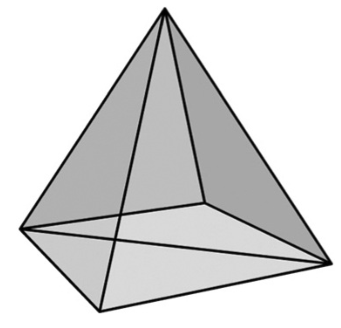
\includegraphics[width=\textwidth]{6-8}
    \centering
    \caption{金字塔三角形}
    \label{fig:6-8}
\end{figure}
%---------- 5 ----------------
\begin{flushleft}
5. 运行“Box” DEMO,并回想一下我们仅在顶点指定颜色。 解释如何为三角形上的每个像素获取像素颜色。\\
解:(猜测)在像素着色阶段时,使用了多采样技术(具体见 4.1.7节),取像素平均值。由于 Box 所使用的颜色简单,多采样使用 1 倍采样做处理即可。(d3dApp.h中m4xMsaaState默认为false)
\end{flushleft}

%---------- 6 ----------------
\begin{flushleft}
6. 修改 Box Demo, 在转换为世界空间之前将以下变换应用于顶点着色器中的每个顶点。
\end{flushleft}
\begin{lstlisting}
vin.PosL.xy += 0.5f*sin(vin.PosL.x)*sin(3.0f*gTime);
vin.PosL.z *= 0.6f + 0.4f*sin(2.0f*gTime);
\end{lstlisting}
\begin{flushleft}
您需要添加一个gTime常量缓冲区变量; 此变量对应于当前的 GameTimer::TotalTime() 值。 使用正弦函数周期性地扭曲顶点来将时间通过顶点动画来展现。\\
解:根据要求作如下修改:
\end{flushleft}
\begin{lstlisting}
// BoxApp.cpp 结构声明 ObjectConstants
struct ObjectConstants
{
    XMFLOAT4X4 WorldViewProj = MathHelper::Identity4x4();
    float gTime; // 新增一个 gTime 属性
};

// BoxApp.cpp BoxApp::Update 增加一行 gTime 赋值语句
void BoxApp::Update(const GameTimer& gt)
{
    //...code...
    objConstants.gTime = mTimer.TotalTime();
    mObjectCB->CopyData(0, objConstants);
}

// BoxApp.cpp BoxApp::BuildConstantBuffers 
// 将 UploadBuffer elementCount 参数改为 2
void BoxApp::BuildConstantBuffers()
{
    mObjectCB = std::make_unique<UploadBuffer<ObjectConstants>>(
                    md3dDevice.Get(), 2, true);

    //...code...
}

// color.hlsl 修改 cbPerObject 结构
cbuffer cbPerObject : register(b0)
{
    float4x4 gWorldViewProj;
    float gTime;
};

// color.hlsl 修改 VS
VertexOut VS(VertexIn vin)
{
    vin.PosL.xy += 0.5f*sin(vin.PosL.x)*sin(3.0f*gTime);
    vin.PosL.z *= 0.6f + 0.4f*sin(2.0f*gTime);

    VertexOut vout;

    // Transform to homogeneous clip space.
    vout.PosH = mul(float4(vin.PosL, 1.0f), gWorldViewProj);
    
    // Just pass vertex color into the pixel shader.
    vout.Color = vin.Color;

    return vout;
}
\end{lstlisting}

%---------- 7 ----------------
\begin{flushleft}
7. 将box和金字塔的顶点(练习4)合并到一个大的顶点缓冲区中。 还将框和金字塔的索引合并到一个大索引缓冲区中(但不更新索引值)。 然后使用 ID3D12CommandList::DrawIndexedInstanced 的参数逐个绘制框和金字塔。 使用世界变换矩阵,使box和金字塔在世界空间中不相交。//
~\\
解:重点在常量缓冲区的更新,设置两个常量缓冲区,构建好各自的 D3D12_CONSTANT_BUFFER_VIEW_DESC,分别代表box 和 pyramid 的 worldViewProj 再做渲染
SetGraphicsRootDescriptorTable 绑定不同的根参数到
\end{flushleft}

%---------- 8 ----------------
\begin{flushleft}
8. 通过在线框(wireframe)模式下渲染多维数据集来修改Box演示。
\end{flushleft}

%---------- 9 ----------------
\begin{flushleft}
9. 修改Box演示, 禁用背面剔除(D3D12\_CULL\_NONE); 也尝试剔除正面而不是背面(D3D12\_CULL\_FRONT)。 以线框(wireframe)模式输出结果,以便您可以更轻松地查看差异。
\end{flushleft}

%---------- 10 ----------------
\begin{flushleft}
10. 如果顶点内存很重要,那么从128位颜色值减少到32位颜色值可能是值得的。修改“Box”演示 在顶点结构中使用32位颜色值而不是128位颜色值。 您的顶点结构和相应的顶点输入描述将如下所示:\\
\end{flushleft}
\begin{lstlisting}
struct Vertex
{
    XMFLOAT3 Pos;
    XMCOLOR Color;
}

D3D12_INPUT_ELEMENT_DESC vertexDesc[] = {
    {“POSITION”, 0, DXGI_FORMAT_R32G32B32_FLOAT, 0, 0, 
                 D3D12_INPUT_PER_VERTEX_DATA, 0},
    {“COLOR”,    0, DXGI_FORMAT_B8G8R8A8_UNORM, 0, 12,
                 D3D12_INPUT_PER_VERTEX_DATA, 0}
};
\end{lstlisting}
\begin{flushleft}
我们使用 DXGI\_FORMAT\_B8G8R8A8\_UNORM 格式(8位红色,绿色,蓝色和alpha)。 此格式对应于常见的32位图形颜色格式ARGB,但 DXGI\_FORMAT 符号以小端表示法列出它们在内存中出现的字节。 在little-endian中,多字节(multi-byte)数据字(word)的字节从最低有效字节写入最高有效字节,这就是为什么 ARGB 在内存中出现为 BGRA,其中最小内存地址处的最低有效字节和最高有效字节为 最高的内存地址。
\end{flushleft}

%---------- 11 ----------------
\begin{flushleft}
11. 思考下面 C++ 顶点结构:
\end{flushleft}
\begin{lstlisting}
struct Vertex
{
    XMFLOAT3 Pos;
    XMFLOAT4 Color;
};
\end{lstlisting}
\begin{itemize}
  \item 1. 输入布局描述顺序是否需要匹配顶点结构顺序? 也就是说,以下顶点声明是否适用于此顶点结构? 做一个实验来找出答案。 然后给出你为什么认为它有效或无效的推理。
  \begin{lstlisting}
  D3D11_INPUT_ELEMENT_DESC vertexDesc[] =
  {
      {“COLOR”,    0, DXGI_FORMAT_R32G32B32A32_FLOAT, 0, 12,
                   D3D11_INPUT_PER_VERTEX_DATA, 0},
      {“POSITION”, 0, DXGI_FORMAT_R32G32B32_FLOAT, 0, 0,
                   D3D11_INPUT_PER_VERTEX_DATA, 0}
  };
  \end{lstlisting}
  \item 2. 相应的顶点着色器结构顺序是否需要匹配 C++ 顶点结构顺序? 也就是说,以下顶点着色器结构是否与上述 C++ 顶点结构一起使用? 做一个实验来找出答案。 然后给出你为什么认为它有效或无效的推理。
  \begin{lstlisting}
  struct VertexIn
  {
      float4 Color : COLOR;
      float3 Pos   : POSITION;
  };
  \end{lstlisting}
\end{itemize}

%---------- 12 ----------------
\begin{flushleft}
12. 将视口(viewport)设置为后缓冲区(back buffer)的左半部分。
\end{flushleft}

%---------- 13 ----------------
\begin{flushleft}
13. 使用剪刀测试来剔除以后缓冲区为中心的矩形外的所有像素,宽度为mClientWidth/2,高度为 mClientHeight/2。 请记住,您还需要使用光栅化器状态组启用剪刀测试。
\end{flushleft}

%---------- 14 ----------------
\begin{flushleft}
14. 像素着色器颜色色调。 使用常量缓冲区为颜色随时间变化。 使用平滑缓动功能。 在顶点着色器和像素着色器中执行此操作。
\end{flushleft}

%---------- 15 ----------------
\begin{flushleft}
15. 修改 Box DEMO 中的像素着色器为如下形式:
\end{flushleft}
\begin{lstlisting}
float4 PS(VertexOut pin) : SV_Target
{
    clip(pin.Color.r - 0.5f);
    return pin.Color;
}
\end{lstlisting}
\begin{flushleft}
运行程序并猜测内置 clip 方法的作用。
\end{flushleft}

%---------- 16 ----------------
\begin{flushleft}
修改 Box 演示中的像素着色器,以在插值顶点颜色和通过常量缓冲区指定的 gPulseColor 之间平滑脉冲。 您还需要更新应用程序端的常量缓冲区。 HLSL代码中的常量缓冲区和像素着色器应如下所示:
\end{flushleft}
\begin{lstlisting}
cbuffer cbPerObject : register(b0)
{
    float4x4 gWorldViewProj;
    float4 gPulseColor;
    float gTime;
};

float4 PS(VertexOut pin) : SV_Target
{
    const float pi = 3.14159;

    // Oscillate a value in [0,1] over time using a sine functio.
    float s = 0.5f*sin(2*gTime - 0.25f(pi) + 0.5f;

    // Linearly interpolate between pin.Color and gPulseColor based on
    // parameter s.
    float4 c = lerp(pin.Color, gPulseColor, s);
    return c;
}
\end{lstlisting}
\begin{flushleft}
gTime 变量对应于 GameTimer::TotalTime() 的值。
\end{flushleft}
